%%%%%%%%%%%%%%%%%%%%%%%%%%%%%%%%%%%%%%%%%%%%%%%%%%%%
% This will help you in writing your homebook
% Remember that the character % is a comment in latex
%
% chapter 1

%%%%%%%%%%%%%%%%%%%%%%%%%%%%%%%%%%%%%%%%%%%%%%%%%%%%%%%%%%%
% you can organize a chapter using sections -> \section{Simulating an inverter}
% or subsections -> \subsection{simulating a particular type of inverter}

%%%%%%   First section

\chapter{Report on the activities held}
\begin{table}[h]
	\begin{tabular}{p{2.1cm}|  p{13.5cm}}
\multicolumn{2}{p{15.0cm}}{ \LARGE{{Setting up the group and the environment to work in team}}}\\
\hline \hline 
\multicolumn{2}{p{1.0cm}}{ \Large{{}}}\\
	07/03/2017 & \textbf{Group formation and selecting the homework}\\
	12/03/2017& Discussing the possibility to work in a team of 4 people, and the preference of the homework available. \\
	\multicolumn{2}{p{1.0cm}}{ \Large{{ }}}\\	
	15/03/2017 & \textbf{Confirmation of the group}	 \\
	&It has been announced the groups and the related project. Another member joined the team. \\
	&We also exchanged the email address and the telephone number to fasten the communication between members abroad (Whatsapp, Skype, Telegram...).\\
		\multicolumn{2}{p{1.0cm}}{ \Large{{ }}}\\
		22/03/2017 & \textbf{Redmine platform}\\
		27/03/2017& Set-up the Redmine platform. Understanding how to use it, register, open a new topic, upload file, register time. \\
		\multicolumn{2}{p{1.0cm}}{ \Large{{ }}}\\	

\end{tabular}
\end{table}	
\begin{table}[h]
	\begin{tabular}{p{1.9cm}|  p{13.5cm}}	
	\multicolumn{2}{p{15.0cm}}{ \LARGE{{Understanding the environment and the requirements}}}\\
	\hline \hline 
	\multicolumn{2}{p{1.0cm}}{ \Large{{}}}\\
	22/03/2017 & \textbf{SEcube documentation}\\
	03/04/2017& Reading the SEcube documentation and write down the analysis.\\
	\multicolumn{2}{p{1.0cm}}{ \Large{{ }}}\\		
	03/04/2017 & \textbf{Communication Protocol v.1.0}\\
	10/04/2017& Meeting with the professor on $ 3^{rd} $ April and on $ 4^{th} $ April. Then we discussed with other projects team (project 13, 7, 14) to enhance the protocol.
	\\ \multicolumn{2}{p{1.0cm}}{ \Large{{ }}}\\	
		11/04/2017 & \textbf{Communication Protocol v.2.0}\\
		20/04/2017 & During Easter Holyday, the project 13 sent the second version to the teacher, but other modifications were needed.\\
		\multicolumn{2}{p{1.0cm}}{ \Large{{ }}}\\	
		26/04/2017 & \textbf{Communication Protocol v.3.0}\\
		02/05/2017 & Discussion with the team involved. Then the project 13 submitted the final protocol.
\end{tabular}
\end{table}	
\begin{table}
	\begin{tabular}{p{2.1cm}|  p{13.5cm}}
		\multicolumn{2}{p{15.0cm}}{ \LARGE{{Project Development and Documentation}}}\\
		\hline \hline 
		\multicolumn{2}{p{1.0cm}}{ \Large{{}}}\\
		18/04/2017 & \textbf{GIT setup and backbone in VHDL}\\
		23/04/2017& Read GIT manual, GIT set up.\\
		 &Write in VHDL the interface of all the components.\\
		\multicolumn{2}{p{1.0cm}}{ \Large{{ }}}\\	
		21/04/2017 & \textbf{Presentation of the $ 26^{th} $ April}	 \\
		26/04/2017 & It has been requested 3 slides talking about:\\
		& \quad- Gantt\\
			&\quad- Milestones - Deliverables\\
			&\quad- Issues already closed - still open..\\

	\multicolumn{2}{p{1.0cm}}{ \Large{{}}}\\
		02/05/2017 & \textbf{Developemnt of the IP-core Manager and documentation}\\
		10/06/2017&-Split the work among us\\
			& - Deciding the communication among the components\\
			& - Write down the architecture, upload it on GIT, perform some tests\\
			& - Report timing and area and synthesys results with LATTICE Diamond\\
			& - Documentation and presentation\\
	%	10/06/2017& We discussed how to split the work among us, if there were any problem between the communication between some components.\\
	%	&We then wrote the architecure in VHDL, upload it on GIT, do some test, write some documentations and presentation.\\
	%	&Finally we tried to some synthesys on the LATTICE Diamond software and tried to the source file on the board.\\
		\multicolumn{2}{p{1.0cm}}{ \Large{{ }}}\\	
		
	\end{tabular}
\end{table}

\begin{figure}[h!]
	\centering	
	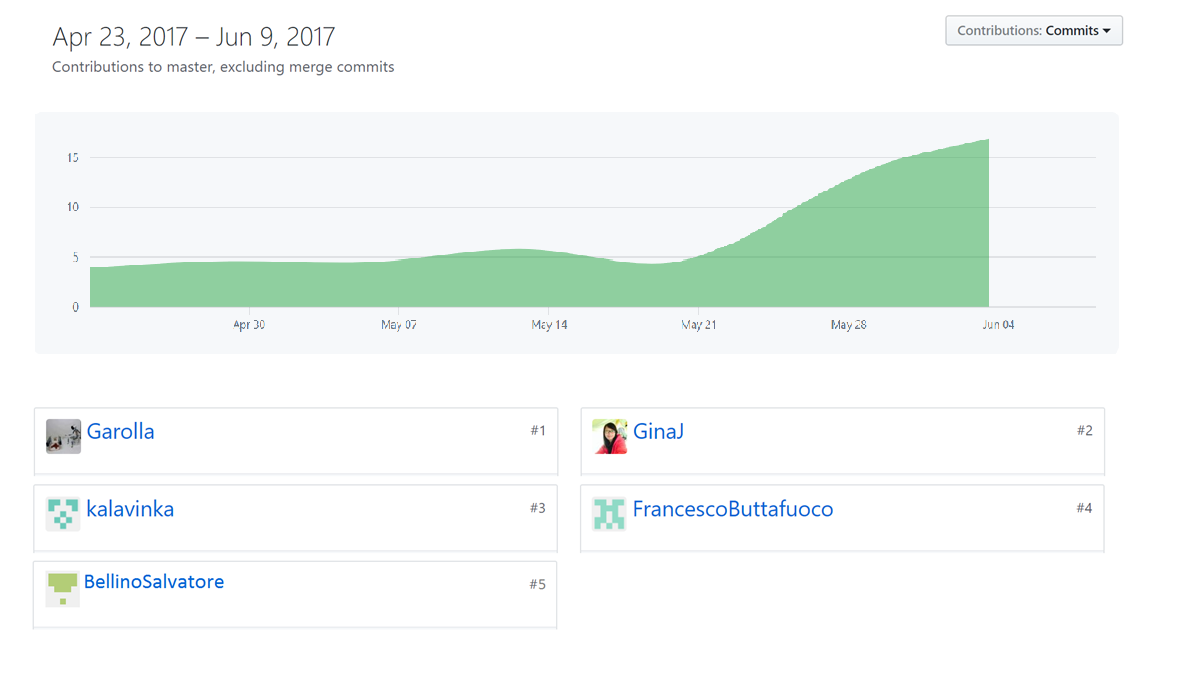
\includegraphics[width=\textwidth]{chapters/git.png}  
	\caption{Our project on GIT, with us as contributors} 
	\label{git}
\end{figure}	
\begin{table}
	\begin{tabular}{p{3.5cm}|  p{12.1cm}}
		\multicolumn{2}{p{15.0cm}}{ \LARGE{{Assignment of the tasks }}}\\
		\hline \hline 
		\multicolumn{2}{p{1.0cm}}{ \Large{{}}}\\
		GAROLLA Emanuele& -Backbone of project in VHDL\\
		& -Dual port buffer 64x16 (Behavioral)\\
		&-Assemble all files\\	
	 &-Final Testbench of the overall architecture	 \\
		 & -Slides\\
		
		\multicolumn{2}{p{1.0cm}}{ \Large{{}}}\\
		JIANG Gina& -Documentation for the $ 26^{th} $ April\\
		&-Documentation for the $ 27^{th} $ May\\
		&-Report timing and area, synthesys result (LATTICE Diamond)\\
		&-Technical report\\
		\multicolumn{2}{p{1.0cm}}{ \Large{{ }}}\\
		
		BELLINO Salvatore& -Dual port buffer 64x16 (Behavioral)\\
		&\qquad -Register 0\\
		&\qquad -Register 16 bits\\
		&\qquad -Decoder\\
		&-Testbench for the data buffer\\
		&-Slides	\\
			
%			\end{tabular}
%		\end{table}	
%		\begin{table}
%			\begin{tabular}{p{3.5cm}|  p{12.1cm}}
%					\multicolumn{2}{p{15.0cm}}{ \%LARGE{{Assignment of the tasks (part 2/2)}}}\\
%					\hline \hline
\multicolumn{2}{p{1.0cm}}{ \Large{{ }}}\\	
		FORNO Evelina& -Dummy IP-core\\
		&-Adder IP-core (FSM with 3 stage)\\
		&-First version of testbench\\
		&-Slides\\
		\multicolumn{2}{p{1.0cm}}{ \Large{{ }}}\\
		BUTTAFUOCO & -IP-Manager Behavioral\\
		Francesco&\qquad-Enabling the right IP core\\
		&\qquad-Propagate the right Data from the selected IP core to the Buffer/CPU\\
		&\qquad-Interrupt Handler\\
		&-Slides\\	
	\end{tabular}
\end{table}
\begin{figure}[h!]
	\centering	
	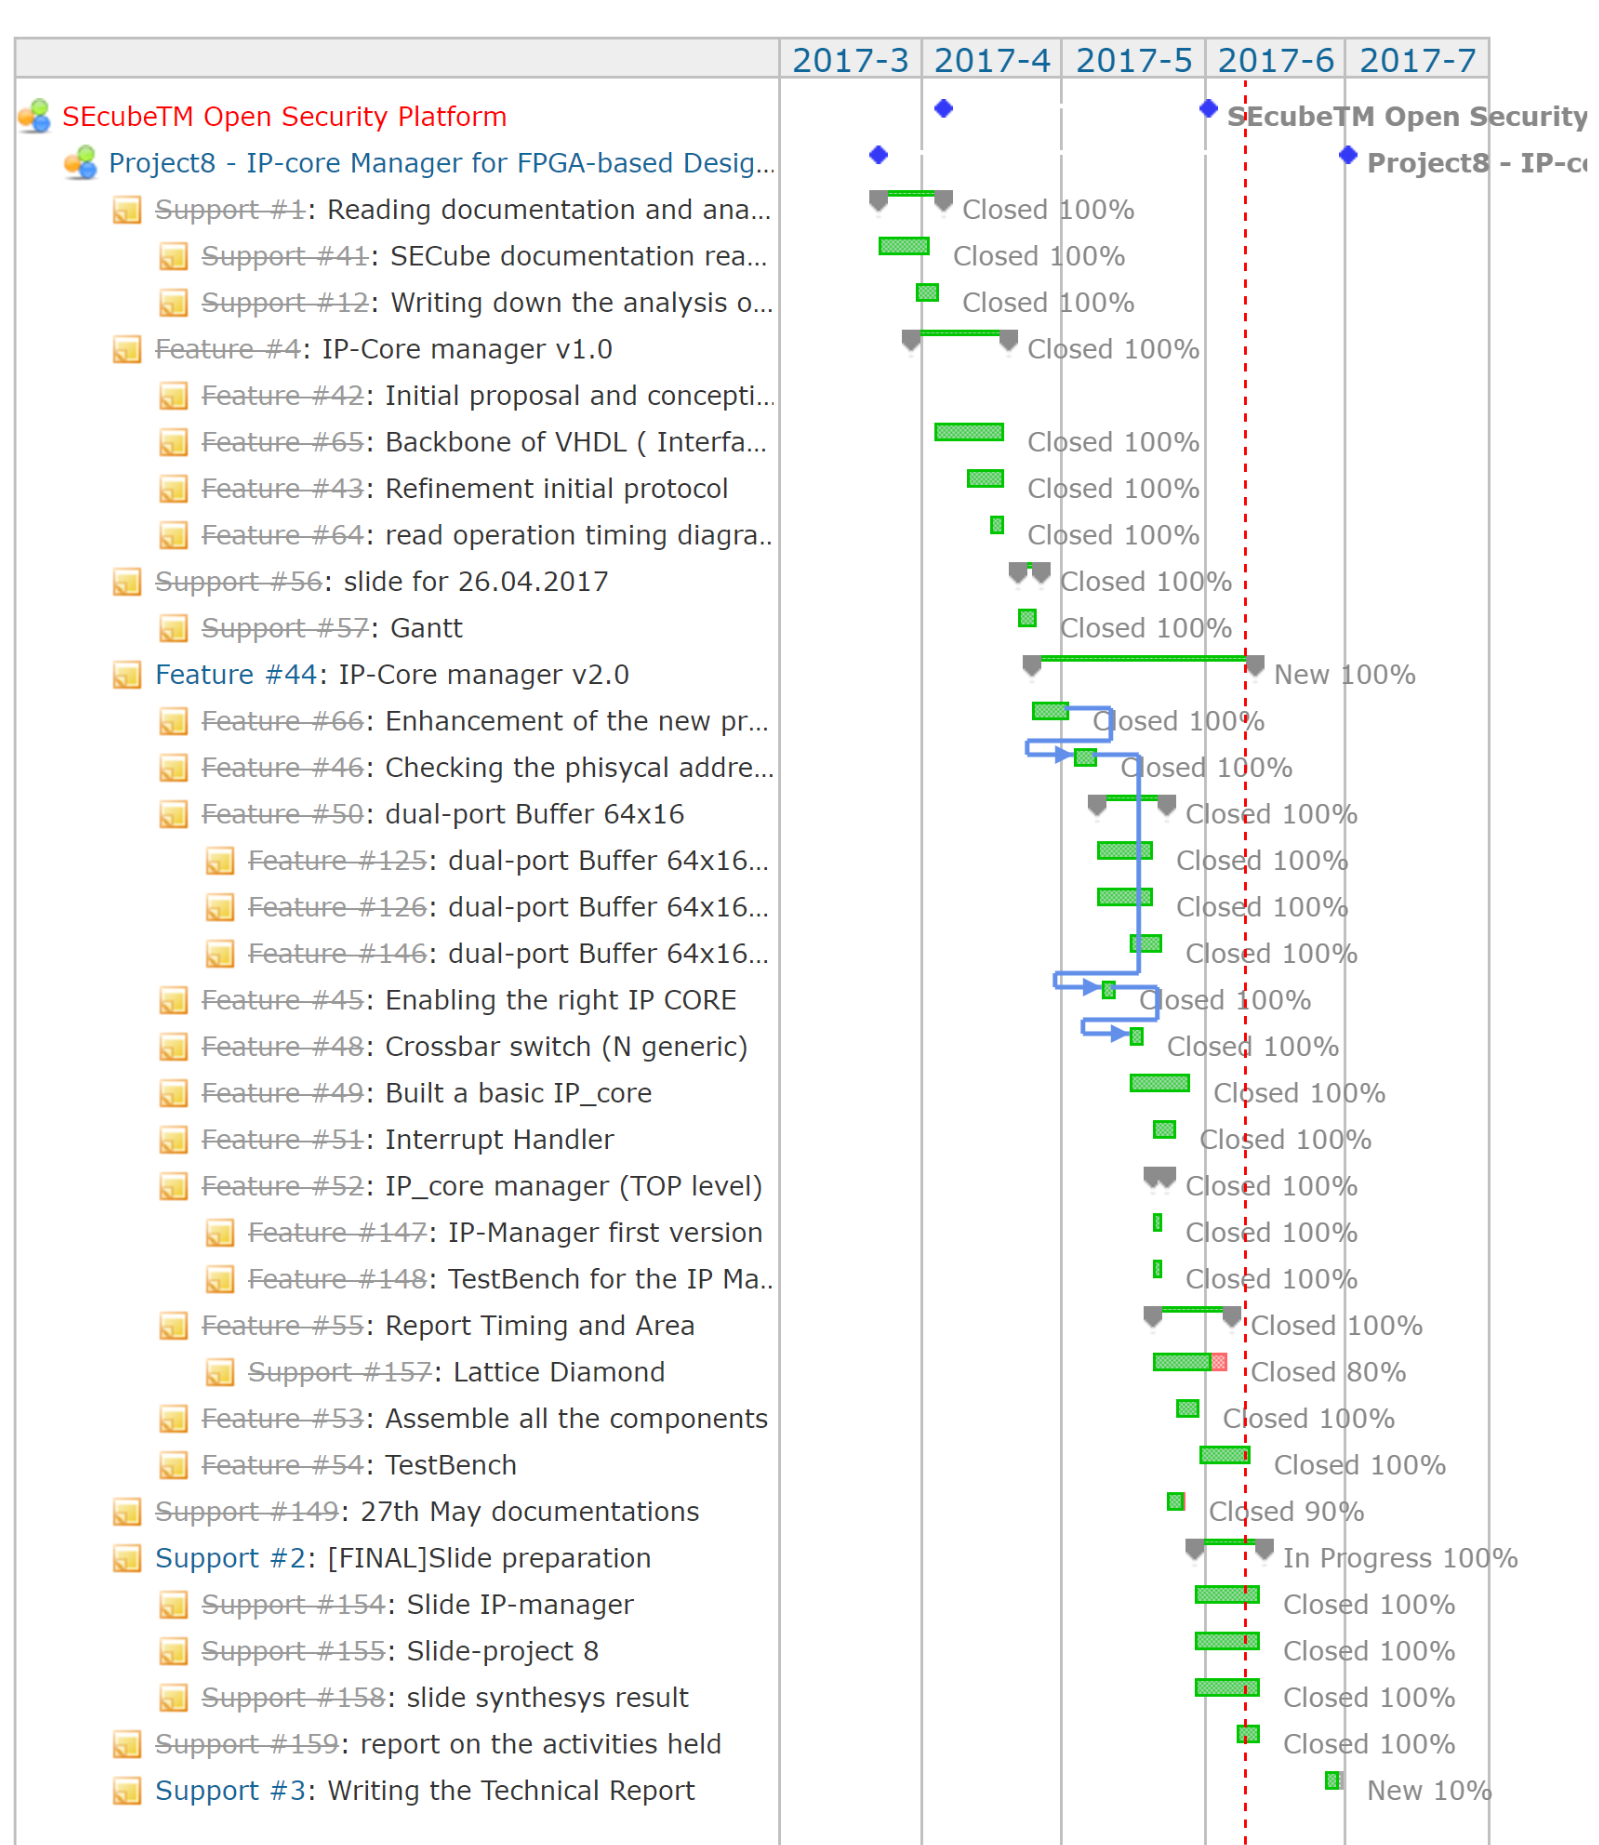
\includegraphics[height=0.65 \textheight]{chapters/gantt.png}  
	\caption{Gantt chart of our project} 
	\label{gantt}
\end{figure}	